\documentclass{beamer}

% fontspecとunicode-mathはLuaLaTeX(XeLaTeX)専用
%\usepackage[no-math]{fontspec}
%\usepackage[math-style=ISO, bold-style = ISO]{unicode-math}
%\setmathfont{Libertinus Math}
%\setmainfont{Libertinus Serif}
%\setsansfont{Libertinus Sans}

\usepackage{libertinus}
\usepackage[T1]{fontenc}

\usepackage{multimedia}

\author{Takumi Noguchi}
\institute{Somewhere}
\date{2021/09/24}

\begin{document}
\begin{frame}
	\maketitle
\end{frame}

% \movie[option]{poster text}{movie file} の書式

\begin{frame}{movie sample (in PDF)}
	\centering
	\movie[width=8cm, height=4.5cm]{%
		% ここがサムネ(テキストでも図でも可)
		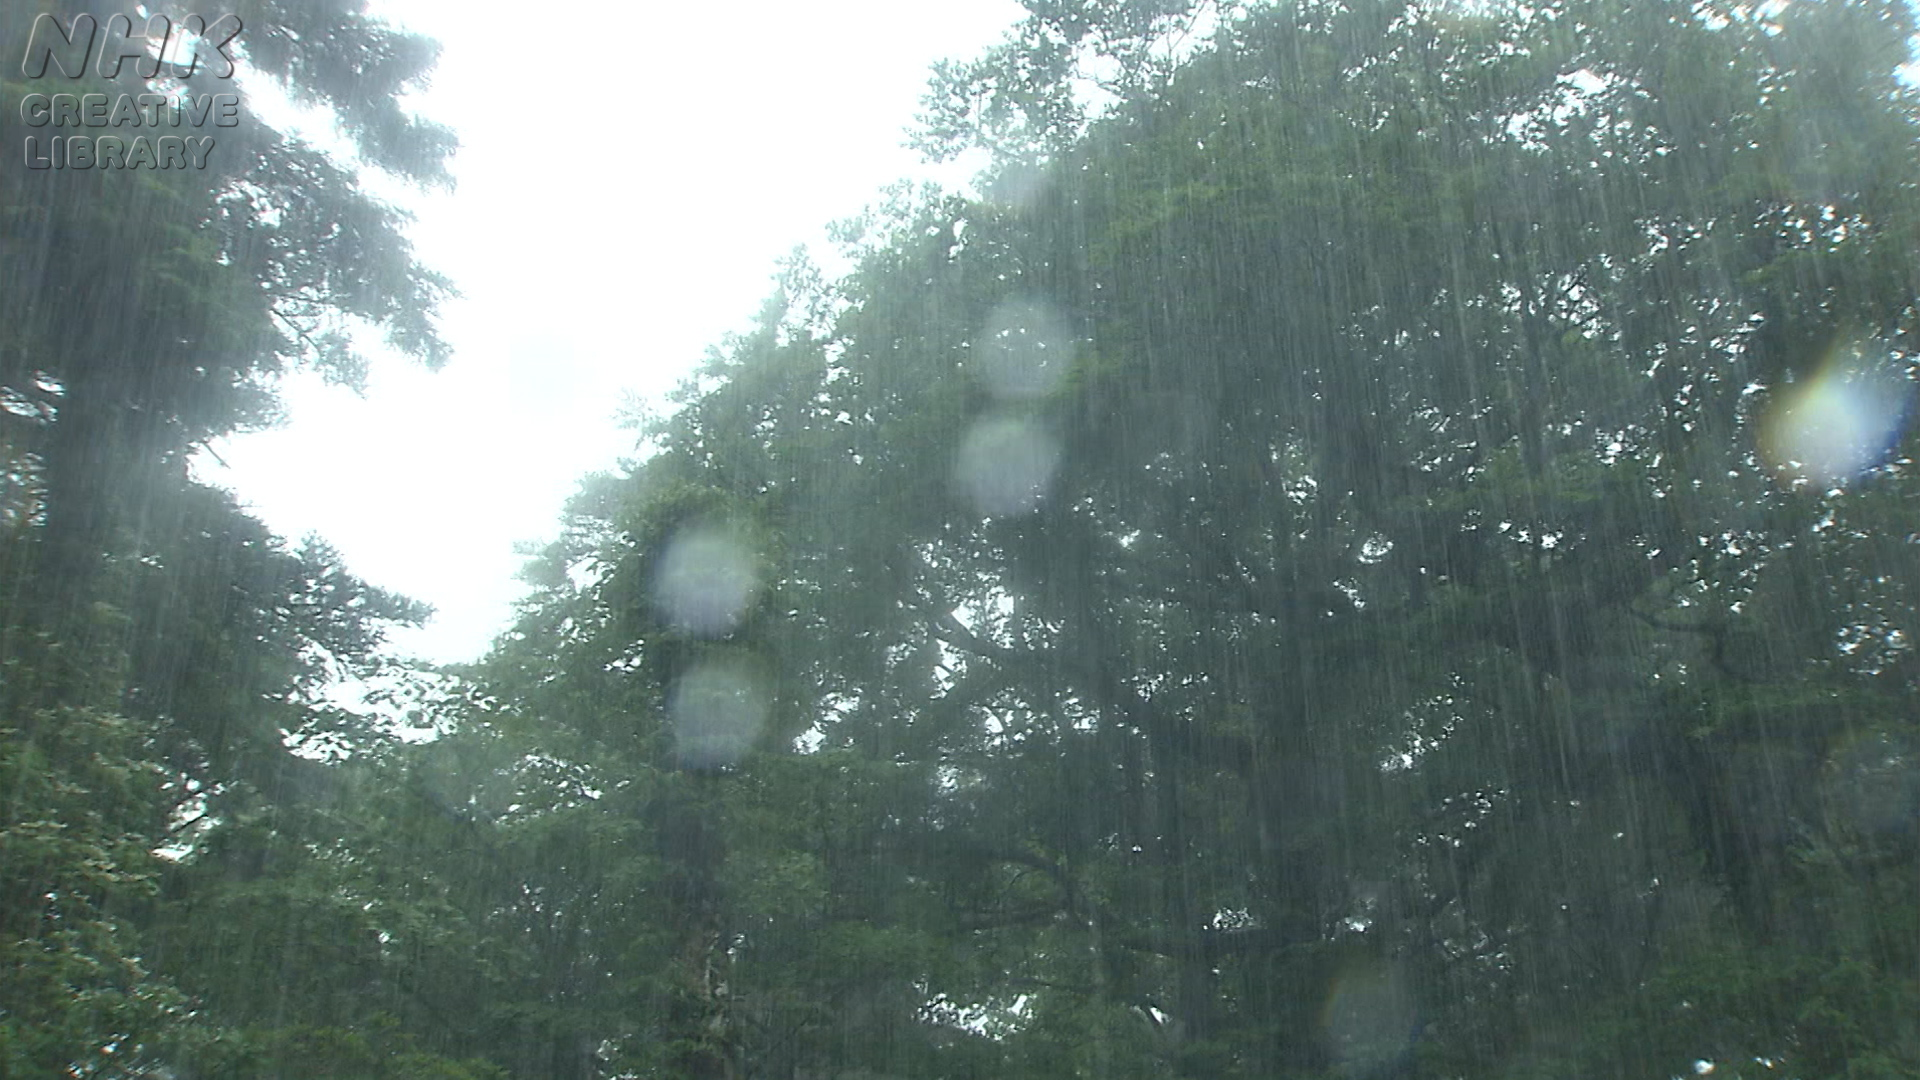
\includegraphics[width=8cm, height=4.5cm]{./fig/sample.jpg}%
	}{./movie/sample.mp4}
\end{frame}

\begin{frame}{movie sample (in external viewer)}
	\centering
	\movie[externalviewer]{
		Click to start the movie
	}{./movie/sample.mp4}
\end{frame}
\end{document}